\documentclass[11pt,pdftex,portrait,letterpaper]{article}
\usepackage[hdivide={1in,*,1in},
            vdivide={1in,*,1in},
%            showframe
            ]{geometry}

\usepackage{graphicx}
\usepackage{longtable}
\usepackage{acronym}
\usepackage{verbatim}
\usepackage{subfigure}
\usepackage{fancyhdr}
\pagestyle{fancy}
\usepackage{listings}
\usepackage{color}
\usepackage{lastpage}

% Default margins are too wide all the way around. Reset them here
\setlength{\topmargin}{-.5in}
\setlength{\textheight}{9in}
\setlength{\oddsidemargin}{.125in}
\setlength{\textwidth}{6.25in}

\lhead{ECEN 898}
\chead{}
\rhead{\thepage\ of \pageref{LastPage}}
%\lfoot{\hline}
\lfoot{}
\cfoot{\small{University of Nebraska - Lincoln Department of Electrical Engineering}}
\rfoot{}
\renewcommand{\footrulewidth}{0.5pt}


% Modify parameters of Listings
\lstset{ 
language=C,
basicstyle=\scriptsize,
numbers=left,
numberstyle=\footnotesize,
stepnumber=1,
numbersep=10pt,
backgroundcolor=\color{white},
frame=single,
captionpos=b,
breaklines=true,
breakatwhitespace=false
}

\begin{document}

\vspace*{30ex}
\begin{center}

\textbf{Final Project - Fast Fourier Transform }\\

\vspace{4ex}
Introduction to Embedded Systems - University of Nebraska \\

\vspace{4ex}
Zach Swanson\\

\end{center}


\pagebreak
\tableofcontents
%\pagebreak
%\listoffigures
%\addcontentsline{toc}{section}{{\bf List of Figures}}
\pagebreak


\section{Introduction}

The purpose of this project was to delve deeper into the theory behind the fast Fourier transform (FFT) by implementing a FFT algorithm on the Texas Instruments (TI) TMS320C5535 ezDSP development board. The algorithm used was the radix-2 decimation in time (DIT). The algorithm was compared to the TI DSPLib and MATLAB FFT functions to obtain results.

%%%%%%%%%%%%%%%%%%%%%%%%%%%%%%%%%%%%%%%%%%%%%%%%%%%%%%%%%%

\section{Theory}

\subsection{Discrete Fourier Transform}

\subsection{Fast Fourier Transform}

\subsubsection{Radix-2}

\subsubsubsection{Decimation in Time}

\subsubsubsection{Decimation in Frequency}

\subsubsection{Other Algorithms}

\subsection{Real-Valued Inputs}

%%%%%%%%%%%%%%%%%%%%%%%%%%%%%%%%%%%%%%%%%%%%%%%%%%%%%%%%%%
 
\section{Program Description}

\subsection{Pre-FFT Routines}

\subsection{Indexing Computational Flow}

\subsection{Butterfly Computations}

\subsection{Post-FFT Routines}

%%%%%%%%%%%%%%%%%%%%%%%%%%%%%%%%%%%%%%%%%%%%%%%%%%%%%%%%%%

\section{Results}

 Figures \ref{f:fig1} and \ref{f:fig2} show the output of this project's, TI's, and MATLAB's FFT algorithms for a 3500 Hz and a 4500 Hz sinusoid. respectively. As the figures illustrate, the output of all the algorithms appear to be identical. To 

\begin{figure}[h]
\centering
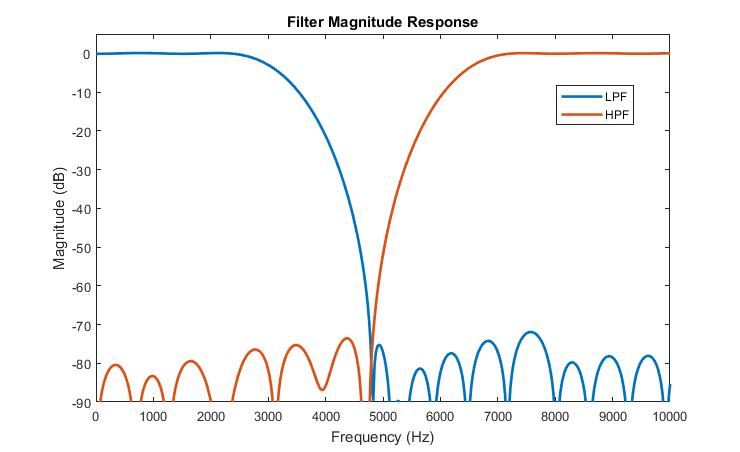
\includegraphics[width=0.8\textwidth]{./filtMag}
\caption{Magnitude response of low- and high-pass filters}
\label{f:fig1}
\end{figure}

\begin{figure}[h]
\centering
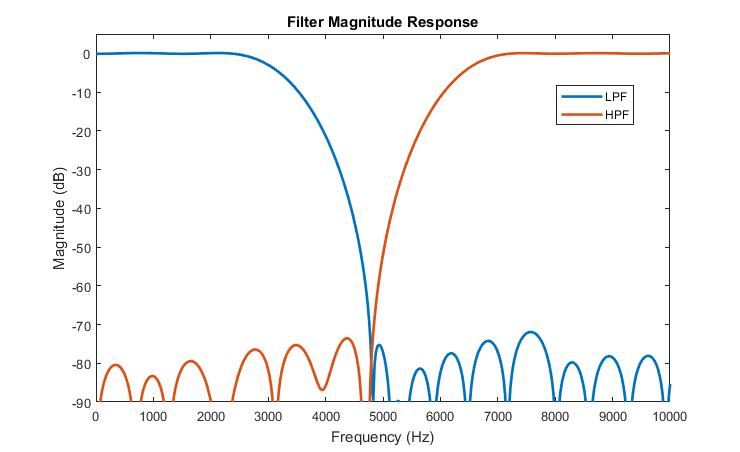
\includegraphics[width=0.8\textwidth]{./filtMag}
\caption{Magnitude response of low- and high-pass filters}
\label{f:fig1}
\end{figure}

%%%%%%%%%%%%%%%%%%%%%%%%%%%%%%%%%%%%%%%%%%%%%%%%%%%%%%%%%%

\section{Conclusion}

\pagebreak

%%%%%%%%%%%%%%%%%%%%%%%%%%%%%%%%%%%%%%%%%%%%%%%%%%%%%%%%%%

\section{Appendix}

Listing \ref{l:code1}

\begin{lstlisting}[caption={FFT and magnitude calculation}, label=l:code1]

\end{lstlisting}

